\documentclass{standalone}
\usepackage{tikz}

\begin{document}

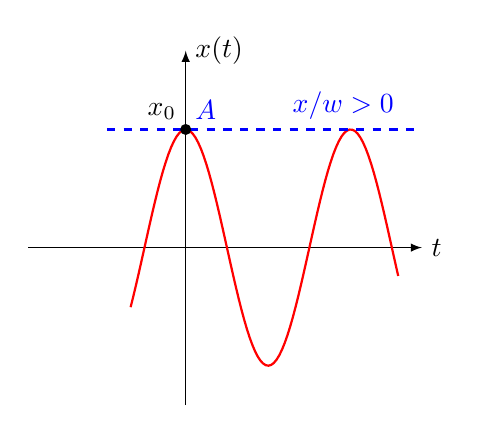
\begin{tikzpicture}[>=latex]
	\draw [->] (-2,0) -- (3,0) node [right] {\(t\)};
	\draw [->] (0,-2) -- (0,2.5) node [right] {\(x(t)\)};
	\draw [thick , red, domain=-0.7:2.7, samples= 100] plot(\x , {1.5*cos(3*\x r)});
	\draw [thick , blue, dashed] (-1,1.5) --++ (4,0);
	\fill (0,1.5) circle (2pt) node [above left] {\(x_0\)};
	\node [above right , blue] at (0,1.5) {\(A\)};
	\node [above, blue] at (2,1.5) {\(x/w>0\)};
\end{tikzpicture}

\end{document}
